\documentclass[border=4pt]{standalone}
\usepackage{tikz}
\usepackage{pgfplots}
\pgfplotsset{compat=1.18}
\usetikzlibrary{shapes.geometric,arrows.meta,positioning,fit,calc,decorations.pathreplacing}
\usepackage{xcolor}
\definecolor{bestcol}{HTML}{1565C0}
\definecolor{freegreen}{HTML}{2E7D32}
\definecolor{learnblue}{HTML}{1565C0}
\definecolor{fusred}{HTML}{C62828}
\newcommand{\best}[1]{{\color{bestcol}\textbf{#1}}}
\begin{document}
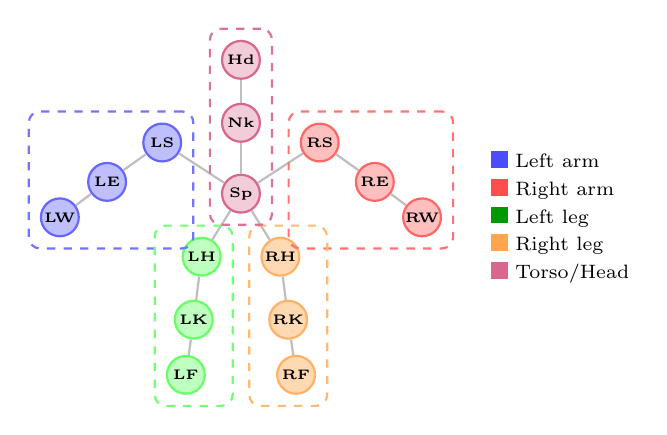
\begin{tikzpicture}[
  every node/.style={font=\scriptsize},
  jnt/.style={circle, draw, minimum size=0.48cm, inner sep=0pt,
              font=\tiny\bfseries, thick},
  la/.style ={jnt, fill=blue!25,   draw=blue!60},
  ra/.style ={jnt, fill=red!25,    draw=red!60},
  ll/.style ={jnt, fill=green!25,  draw=green!60},
  rl/.style ={jnt, fill=orange!30, draw=orange!60},
  tr/.style ={jnt, fill=purple!20, draw=purple!60},
  grp/.style={draw, dashed, rounded corners=4pt, inner sep=4pt, thick},
  sk/.style ={gray!50, thick}
]
%% joints
\node[tr] (sp) at (0,0)     {Sp};
\node[tr] (nk) at (0,0.9)   {Nk};
\node[tr] (hd) at (0,1.7)   {Hd};
\node[la] (ls) at (-1.0,0.65){LS};
\node[la] (le) at (-1.7,0.15){LE};
\node[la] (lw) at (-2.3,-0.3){LW};
\node[ra] (rs) at ( 1.0,0.65){RS};
\node[ra] (re) at ( 1.7,0.15){RE};
\node[ra] (rw) at ( 2.3,-0.3){RW};
\node[ll] (lh) at (-0.5,-0.8){LH};
\node[ll] (lk) at (-0.6,-1.6){LK};
\node[ll] (lf) at (-0.7,-2.3){LF};
\node[rl] (rh) at ( 0.5,-0.8){RH};
\node[rl] (rk) at ( 0.6,-1.6){RK};
\node[rl] (rf) at ( 0.7,-2.3){RF};

%% skeleton edges
\foreach \a/\b in {sp/nk,nk/hd,sp/ls,sp/rs,ls/le,le/lw,rs/re,re/rw,
                   sp/lh,sp/rh,lh/lk,lk/lf,rh/rk,rk/rf}
  \draw[sk] (\a)--(\b);

%% group outlines
\node[grp,draw=blue!55,   fit=(ls)(le)(lw)] {};
\node[grp,draw=red!55,    fit=(rs)(re)(rw)] {};
\node[grp,draw=green!55,  fit=(lh)(lk)(lf)] {};
\node[grp,draw=orange!55, fit=(rh)(rk)(rf)] {};
\node[grp,draw=purple!55, fit=(sp)(nk)(hd)] {};

%% legend (right side)
\node[right=0.5cm of rw, align=left] (leg) {%
  \textcolor{blue!70}{\rule{6pt}{6pt}}~Left arm\\[2pt]
  \textcolor{red!70}{\rule{6pt}{6pt}}~Right arm\\[2pt]
  \textcolor{green!60!black}{\rule{6pt}{6pt}}~Left leg\\[2pt]
  \textcolor{orange!70}{\rule{6pt}{6pt}}~Right leg\\[2pt]
  \textcolor{purple!60}{\rule{6pt}{6pt}}~Torso/Head
};
\end{tikzpicture}
\end{document}
